\documentclass[a4paper]{article}
\usepackage[utf8]{inputenc}
\usepackage[T1]{fontenc}
\usepackage[ngerman]{babel}
\usepackage{ntheorem}
\usepackage{graphicx}
\usepackage{floatrow}
\usepackage{float}
\usepackage{hyperref}

\theoremstyle{break}
\newtheorem{defi}{Definition}[section]
\newtheorem{ex}{Beispiel}[section]
\newtheorem{why}{Vorteile}[section]
\newtheorem{whynot}{Nachteile}[section]
\title{SWT 1: Architekturstile by example}
\author{Adrian E. Lehmann}

\begin{document}
	\maketitle
	\tableofcontents
	\newpage
	

\section{Softwaretypen}
\subsection{Abstrakte Maschine}
Auch virtuelle Maschine oder \textit{engl. Virtual Machine (VM)}
\begin{defi}
	Eine virtuelle Maschine ist eine Menge an Befehlen und Objekten, die auf einer darunter liegenden Maschine aufbauen und diese ganz oder teilweise verdecken
\end{defi}

\begin{ex}
\begin{enumerate}
	\item JVM
	\item KVM / VirtualBox / etc
\end{enumerate}
\end{ex}

\begin{why}
		Man verwendet virtuelle Maschinen um ein System zu kapseln und somit eine kontrollierte Umgebung zu haben. Eine kontrollierte Umgebung hat Vorteile für das Host- sowie das Gastsystem: Das Hostsystem kann unbehelligt weiter arbeiten und es erfolgen keinerlei ungewollte Änderungen durch das Gastsystem auf diesem. Das Gastsystem hingegen kann in seiner 'idealen' Umgebung verwendet werden und kann somit optimal laufen. Weiterhin kann man so Software für mehrere System einfach ausliefern: In dem diese System eine kompatible VM installiert haben, kann die erstelle Software ausgeführt werden (bestes Beispiel: Java)
\end{why}

\subsection{Programmfamilie}
Auch Software-Produktlinie oder \textit{engl. Program Family}
\begin{defi}
	Eine Programmfamilie ist eine Menge von Software welche erhebliche Anteile von Anforderungen, Entwurfsbestandteilen oder Softwarekomponenten gemeinsam verwenden.
	Die Programme einer solchen Familie unterscheiden sich extern durch I/O, Funktionsumfang und der Zielhardware und intern durch evtl. verschiedene Algorithmen und/oder Datenstrukturen.
\end{defi}

\begin{ex}
	\begin{enumerate}
		\item LibreOffice
		\item Creative Cloud
	\end{enumerate}
\end{ex}

\begin{why}
	Auf Grund der Wiederverwendung von Komponenten wird die Entwicklung kürzer und kostengünstiger. Weiterhin werden die Programme hiermit besser wartbar, da man Funktionalitätsupdates an die ganze Produktfamilie 'auf einmal' ausliefern kann.
\end{why}
\newpage
\section{Benötigte Definitionen}
\subsection{Schicht}

\textit{engl. Layer}
\begin{defi}{Schicht}
	Eine Schicht besteht aus Softwarekomponenten, welche durch eine (wohldefinierte) Schnittstelle zur Verfügung gestellt werden.
\end{defi}

Eine Schicht kann wiederum in mehrere sog. Partitionen aufgeteilt werden, welche untereinander auch kommunizieren können. Schichten könne i.A. untereinander nicht kommunizieren (siehe Schichtenarchitektur).

\subsection{Plugin}
\begin{defi}{Plugin}
	Ein Plugin ist ein Einschub in ein Framework, welcher Methoden aus (abstrakten) Oberklassen oder Schnittstellen überschreibt um zusätzliche Funktionalität und/oder Anwendungslogik bereit zu stellen.
\end{defi}
\subsection{Universal Description, Discovery and Integration (UDDI)}
\begin{defi}
	Bezeichnet einen standardisierten Verzeichnisdienst, der die zentrale Rolle in SOA, welcher das Finden und Laden von Diensten unterstützt. Dieser kam aus einer Industrieinitiative von großen Firmen hervor.
\end{defi}
\textbf{Ziele:}
\begin{itemize}
	\item Maximierung der Web-Service-Wiederverwendung
	\item Erzeugung einer Management- und Governance-Struktur
	\item Speicherung aller Metadaten zu einem Web-Service und allen assoziierten Dokumenten
	\item Bereitstellung von flexiblen Verwaltungs- und Zugriffsschnittstellen
	\item Anpassung an sich ändernde Geschäftsanforderungen und eine wachsende Anzahl an Services und Nutzern
\end{itemize}
\section{Architekturstile}
\subsection{Schichtenarchitektur}
\textit{engl. Layered Architecture}

\begin{defi}
	Eine Schichten Architektur glieder Software in einzelne Schichten
\end{defi}
Es gibt mehrere Typen einer Schichtenarchitektur: 
\begin{itemize}
	\item Eine transparente Schichtenarchitektur erlaubt es das jede Schicht auf die Schnittstelle jeder Schicht unter ihr zugreifen darf.
	\item Eine intransparente Schichtenarchitektur erlaubt einer Schicht nur den Zugriff auf die Schnittstelle der Schicht direkt unter ihr selbst.
\end{itemize}

\begin{why}
	\begin{enumerate}
		\item Zur Übersichtlichkeit der Modellierung / der Software
		\item Um Abstraktionsebenen zu definieren
		\item Die Wartbarkeit wird verbessert, da man Schichten einfach gegen andere Implementierungen tauschen kann
		\item Die Wiederverwertbarkeit zwischen Software wird verbessert
		
	\end{enumerate}
\end{why}
\begin{whynot}
	\begin{enumerate}
		\item Schichtenaufteilung manchmal schwierig
		\item Kommunikation u. U. umständlich (gerade bei falls intransparent)
	\end{enumerate}
\end{whynot}
Zur Implementierung siehe das Entwurfsmuster Fassade.


\subsection{Klient / Dienstgeber}
\textit{engl. bzw. allgemein verständlich: Client/Server}
\begin{defi}
	Eine Architektur in welcher ein Dienstgeber einem oder mehreren Klienten Dienste anbietet. Dabei rufen die einzelnen Klienten Funktionen auf dem Dienstgeber auf.
\end{defi}
\begin{itemize}
	\item Der Klient muss die Schnittstelle des Dienstgebers kennen
	\item Umgekehrt ist dies nicht der Fall
\end{itemize}
\begin{ex}
	Ein Dienstgeber bietet häufig ein Datenbankbackend, auf welches die Klienten (meist Applikationen) zugreifen. Beispiele hierfür sind quasi unendlich verfügbar. Das wohl weit verbreitetste sind "WebServer" also Dienstgeber die einem eine Webseite zur Verfügung stellen.
\end{ex}
\begin{why}
	\begin{itemize}
		\item Software kann "geheim" gehalten werden
		\item Schwachen Klienten, wie z.B. Smartphones, kann Arbeit abgenommen werden
	\end{itemize}
\end{why}
\begin{whynot}
	\begin{itemize}
		\item Evtl. viel Rechenleistung nötig und somit teuer
		\item Zentralisierung bietet Angriffsfläche
		\item Datenschutz u. U. fragwürdig
	\end{itemize}
\end{whynot}


\subsection{Partnernetze}
\textit{engl. bzw. allgemein verständlich: Peer to peer (P2P) network}
\begin{defi}
	Eine Verallgemeinerung des Klient Dienstgebersystems, bei dem alle Netzwerkpartner die gleichen Aufgaben und Rechte haben.
\end{defi}
\textbf{Wichtige Eigenschaften:}
\begin{itemize}
	\item Partnernetze sind \textbf{dezentralisiert}
	\item \textbf{Rollensymmetrie}: Alle Partner sind Klient und Dienstgeber zu gleich
	\item \textbf{Selbstorganisation}: Die korrekte Funktionalität und das Verhalten wird durch die Interaktion und durch die Kommunikation der Partner gesteuert
	\item \textbf{Verfügbarkeit}: Alle Daten sind redundant über mehrere Partner verteilt
	\item \textbf{Autonomie}: Jeder Partner arbeitet für sich ohne Einfluss der anderen
	\item \textbf{Zuverlässigkeit}: Ein Partnernetz hat eine hohe Ausfallsicherheit auf Grund der hohen Redundanz
\end{itemize}
\begin{ex}
	\begin{itemize}
		\item Torrent
		\item Dezentrale Kommunikationsdienst (z.B Matrix)
		\item Skype (Teilweise)
		\item Blockchain (z.B. Bitcoin)
	\end{itemize}
\end{ex}
\begin{why}
	\begin{itemize}
		\item Sicherheit
		\item Datenschutz
		\item Lastverteilung
	\end{itemize}
\end{why}
\begin{whynot}
	\begin{itemize}
		\item Notwendige Weitergabe der Software
		\item Leichterer Eindrang für schwarze Schafe (wenn auch gut kontrollierbar)
	\end{itemize}
\end{whynot}



\subsection{Datenablage}
\textit{auch: Depot, engl. bzw. allgemein verständlich: Repository (Repo)}
\begin{defi}
	Eine Datenablage erlaubt es Subsystemen, welche lose gekoppelt sind, die gehaltenen Daten abzurufen und u.U. zu modifizieren und somit über die Datenablage zu interagieren.
\end{defi}
Repos eignen sich für parallelen und sequenziellen Zugriff. Achtung! Bei parallelem Zugriff ist es wichtig Synchronisation zu beachten.
Repos können lokal oder per remote access (Fernzugriff) funktionieren
\begin{ex}
	\begin{itemize}
		\item git
		\item Package manager wie z.B. Aptitude beziehen ihre Daten aus Repos
	\end{itemize}
\end{ex}



\subsection{Model View Controller}
\textit{kurz: MVC}
\begin{defi}
	Die MVC Architektur teilt ein System in drei Teile: Das Modell, die Präsentation und die Steuerung
\end{defi}
\textbf{Hierbei sind:}
\begin{itemize}
	\item \textbf{Modell / \textit{engl. Model}}: Der Teil der Software, welche die Datenhaltung und Datenstruktur verwaltet
	\item \textbf{Präsentation / \textit{engl. View}}: Der Teil der Software, welcher die (u.U. manipulierten) Daten und Objekte darstellt (häufig graphisch)
	\item \textbf{Steuerung / \textit{engl. Controller}}: Der Teil der Software, der für Interaktion zuständig ist: Die Steuerung ändert und liest das Modell und meldet dem View diese Änderungen
\end{itemize}
\begin{ex}
	\begin{itemize}
		\item (Fast) Jede Anwendung mit einer GUI und einem Datenbankbackend  
	\end{itemize}
\end{ex}
\begin{why}
	\begin{itemize}
		\item Simultane Entwicklung der einzelnen Teile möglich
		\item Wenig Kopplung
		\item Leicht zu Modifizieren
		\item Mehrere Views erlauben verschiedene Darstellung der Daten (z.B. CLI \& GUI)
		\item Entwurfsmuster Beobachter gut einsetzbar
	\end{itemize}
\end{why}
\begin{whynot}
	\begin{itemize}
		\item Steile Lernkurve
		\item Sehr saubere Schnittstellenmodellierung nötig
		\item Code wird häufig sehr groß
	\end{itemize}
\end{whynot}
\begin{figure}[H]
	\centering
	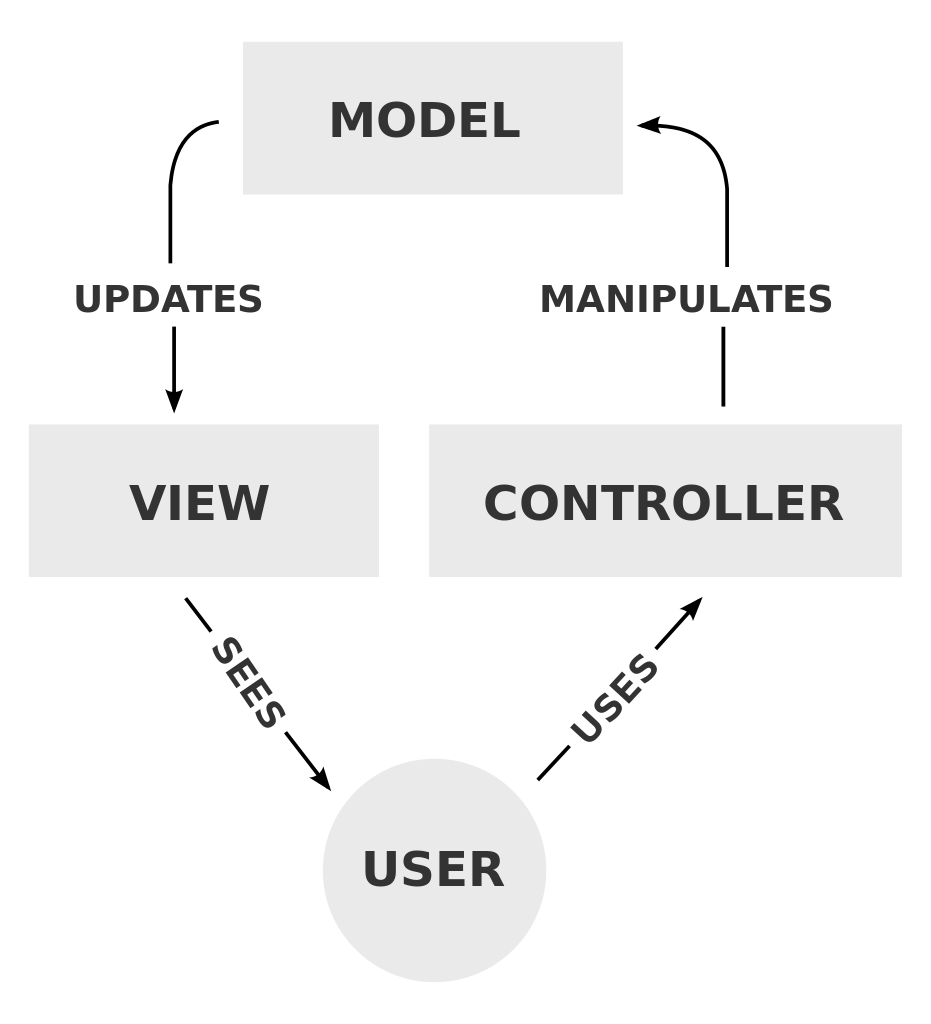
\includegraphics[width=\textwidth]{../diagrams/misc/mvc.png}
	\caption{MVC}
\end{figure}

\subsection{Fließband}
\textit{engl. Pipeline (auch: Pipe)}
\begin{defi}
	Eine Archtitekturstil, bei dem ein Objekt oder eine Menge an Objekten einen Prozess einer endlichen Anzahl Stufen durchläuft, wobei diese Stufe immer eine Datum bzw. eine Menge an Daten verarbeiten, jedoch alle Stufen gleichzeitig operieren
\end{defi}
Um Geschwindigkeitsdifferenzen auszugleichen haben Stufen Pufferspeicher.
\begin{ex}
	\begin{itemize}
		\item Unix shell piping (z.B. aptitude search tex | grep live)
		\item Java Stream operations (Nur teilweise)
	\end{itemize}
\end{ex}
\begin{why}
	\begin{itemize}
		\item Parallelisierung
		\item Bestens nutzbar für Stapelverarbeitung oder Datenstromverarbeitung
	\end{itemize}
\end{why}
\begin{whynot}
	\begin{itemize}
		\item Ungleiche Dauer der einzelnen Stufen können evtl. zu Problemen (trotz Buffer) führen
	\end{itemize}
\end{whynot}
\begin{figure}[H]
	\centering
	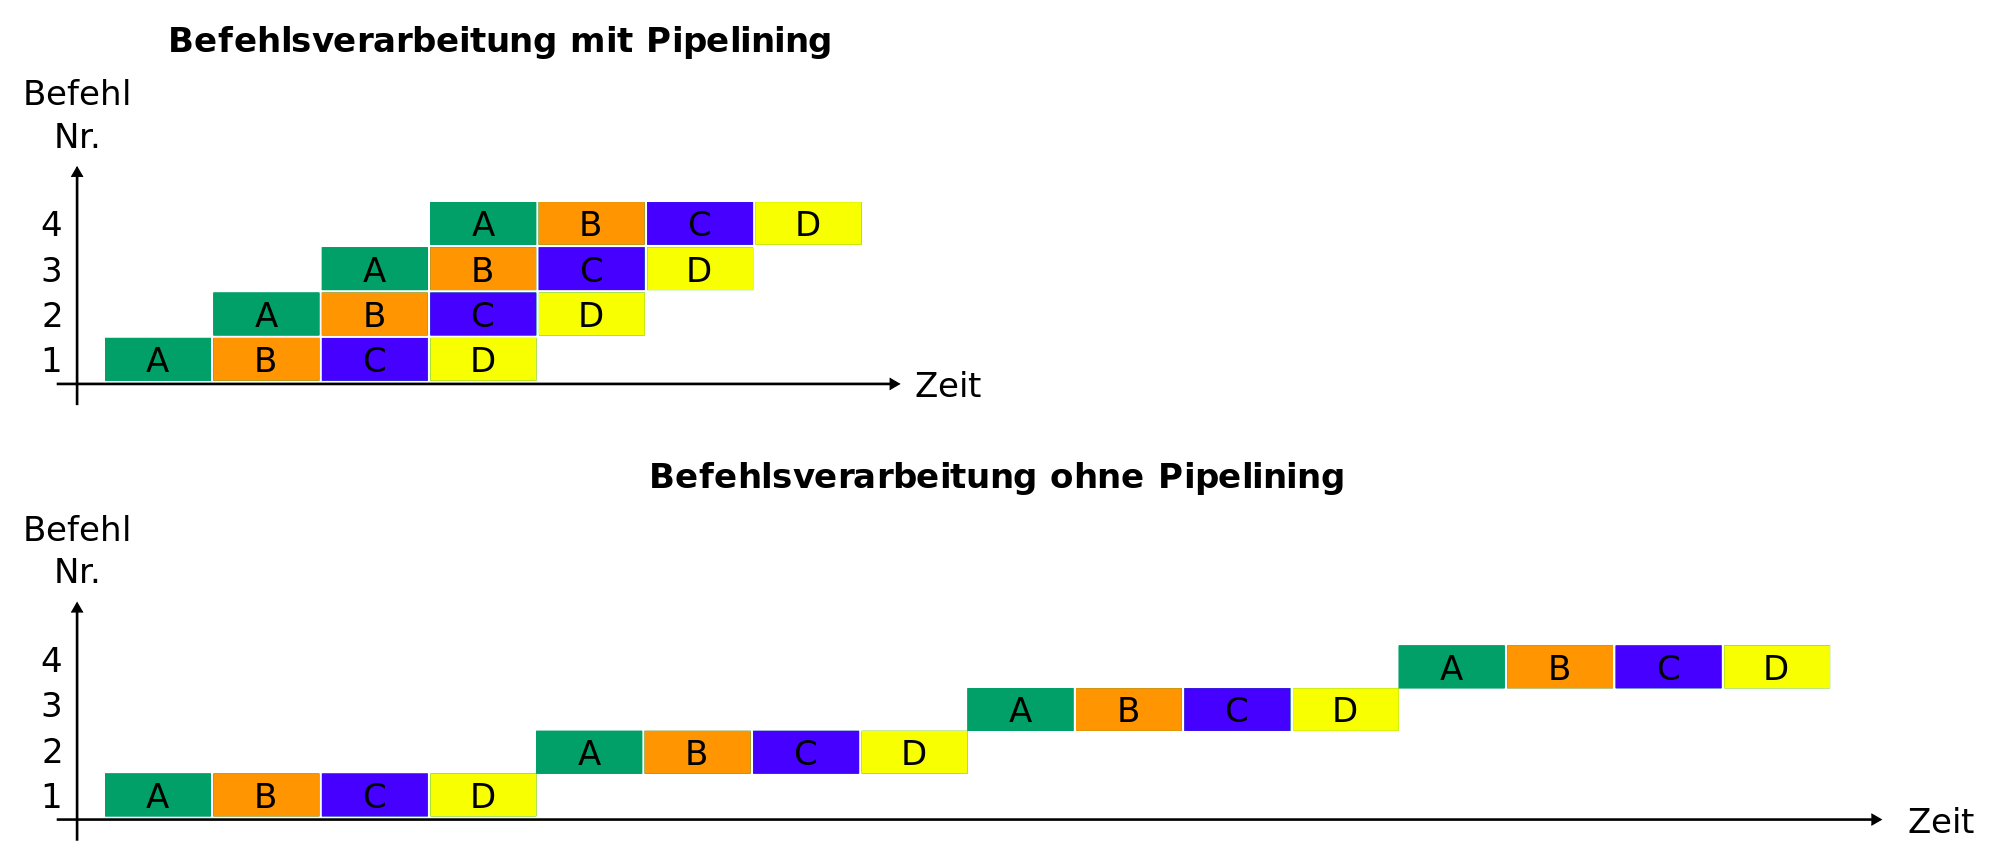
\includegraphics[width=\textwidth]{../diagrams/misc/pipeline.png}
	\caption{Pipeline}
	\floatfoot{Source: (Frank Jacobsen, Commons-Wiki, 14 Jul 2017)}
\end{figure}


\subsection{Rahmenarchitektur}
\textit{engl. Framework}
\begin{defi}
	Eine Rahmenarchitektur bietet ein (fast) vollständiges Programm an, welches konzipiert ist um Lücken zu haben und somit Erweiterungen zuzulassen. Allerdings enthält das Programm die vollständige Anwendungslogik um als selbststehendes Programm agieren zu können.
\end{defi}
Die Einschübe werden auch \textit{Plugins genannt}. Weiterhin benutzt ein Framework das Hollywoodprinzip: "Don't call us; we call you". D.h. Die Rahmenarchitektur ruft die Methoden der plug-ins auf und i.A. nicht umgekehrt.
\begin{ex}
	\begin{itemize}
		\item IntelliJ
		\item Firefox
		\item (jmjrst) \textit{(Bad example - for obv. reasons)}
	\end{itemize}
\end{ex}
\begin{why}
	\begin{itemize}
		\item Grundversion der Anwendung funktoniert
		\item Flexibilität
		\item Wiederverwendbarkeit (z.B. JetBrains basiert viele IDEs auf IntelliJ)
		\item Die Entwurfsmuster Strategie, Fabrikmethode, abstrakte Fabrik und Schablonenmethode sind oft anwendbar
	\end{itemize}
\end{why}
\begin{whynot}
	\begin{itemize}
		\item Teilweise großer Overhead
		\item Änderungen am Grundprogramm können viele Plugins nutzlos machen
	\end{itemize}
\end{whynot}



\subsection{Dienstorientierte Architekturen}
\textit{engl. Service Oriented Architecture (kurz SOA)}
\begin{defi}
	SOA ist ein Architekturstil, bei dem Anwendungen aus (unabhängigen) Diensten (engl. services) zusammengestellt werden. Diese Dienste können über ein Kommunikationsprotokoll kommunizieren.
\end{defi}
Dienste können bei SOA dynamisch zur Laufzeit eingebunden werden. Diese Dienste werden durch UDDI gesucht. 
\begin{why}
	\begin{itemize}
		\item Bereitstellen gekapselter Funktionalität an andere Dienste und Anwendungen
		\item Austauschbarkeit von Diensten
		\item Flexibilität
		\item Lose Kopplung
		\item Offene Standards
	\end{itemize}
\end{why}
\begin{whynot}
	\begin{itemize}
		\item Sehr kompliziert
		\item Testen sehr schwer, durch Service loading
		\item Verwenden von Diensten, die untereinander inkompatibel sind, kann zu Problemen führen.
	\end{itemize}
\end{whynot}
\newpage
\appendix
\section{Quellen}
\begin{itemize}
	\item Folien des IPD, KIT
	\item Gelerntes aus Vorlesung SWT1 durch Prof. Tichy, KIT
	\item Bruegge, Bernd, and Allen H. Dutoit. Object-oriented Software Engineering: Using UML, Patterns, and Java. Harlow (UK): Pearson, 2014. Print. 
\end{itemize}
\end{document}



